\documentclass[10pt]{article}
\usepackage{tikz}
\usepackage[margin=0cm]{geometry}
\pagestyle{empty}

\begin{document}

\vspace*{\fill}
\begin{center}
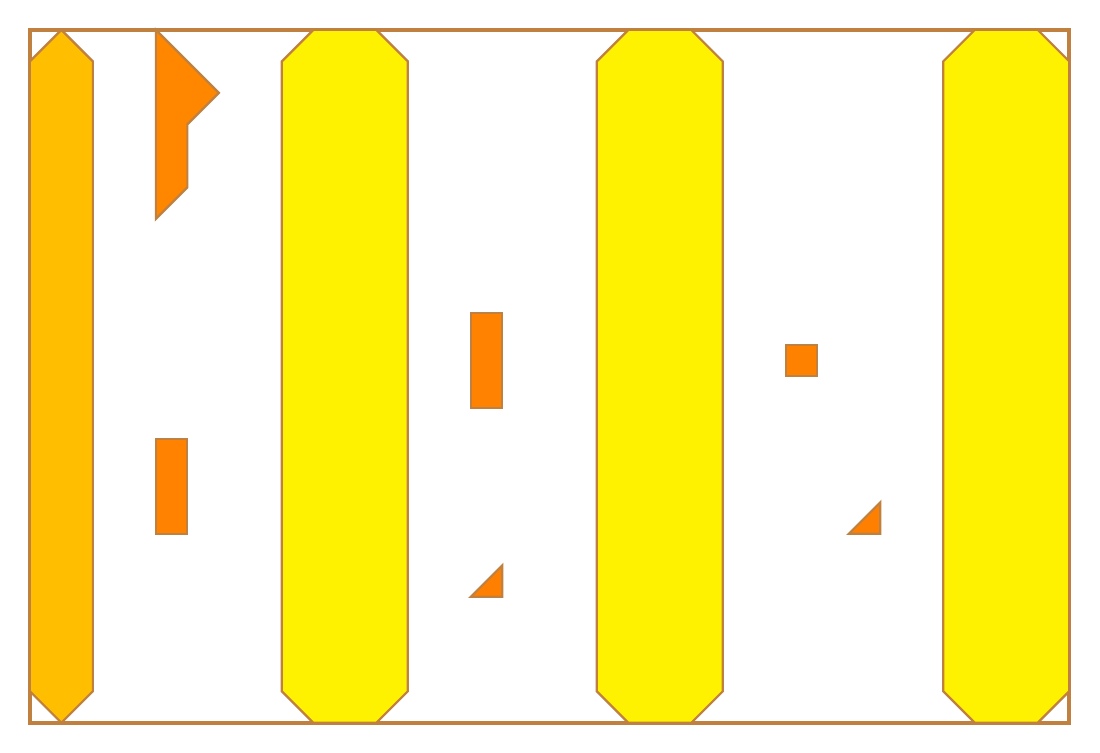
\begin{tikzpicture}[x=0.4cm, y=-0.4cm, thick, brown]
\draw[ultra thick] (0, 0) -- (33, 0) -- (33, 22) -- (0, 22) -- cycle;
%Depth 0
\filldraw[fill=orange!51!yellow] (1, 0) -- (2, 1) -- (2, 21) -- (1, 22) -- (0, 21) -- (0, 1) -- cycle;
\filldraw[fill=orange!94!yellow] (4, 0) -- (6, 2) -- (5, 3) -- (5, 5) -- (4, 6) -- cycle;
\filldraw[fill=orange!0!yellow] (9, 0) -- (11, 0) -- (12, 1) -- (12, 21) -- (11, 22) -- (9, 22) -- (8, 21) -- (8, 1) -- cycle;
\filldraw[fill=orange!0!yellow] (19, 0) -- (21, 0) -- (22, 1) -- (22, 21) -- (21, 22) -- (19, 22) -- (18, 21) -- (18, 1) -- cycle;
\filldraw[fill=orange!0!yellow] (30, 0) -- (32, 0) -- (33, 1) -- (33, 21) -- (32, 22) -- (30, 22) -- (29, 21) -- (29, 1) -- cycle;
\filldraw[fill=orange!97!yellow] (14, 9) -- (15, 9) -- (15, 12) -- (14, 12) -- cycle;
\filldraw[fill=orange!99!yellow] (24, 10) -- (25, 10) -- (25, 11) -- (24, 11) -- cycle;
\filldraw[fill=orange!97!yellow] (4, 13) -- (5, 13) -- (5, 16) -- (4, 16) -- cycle;
\filldraw[fill=orange!100!yellow] (27, 15) -- (27, 16) -- (26, 16) -- cycle;
\filldraw[fill=orange!100!yellow] (15, 17) -- (15, 18) -- (14, 18) -- cycle;
\end{tikzpicture}
\end{center}
\vspace*{\fill}

\end{document}
